\documentclass[11pt]{article}
\usepackage{url}
\usepackage{cite}
\usepackage{amsmath}
\usepackage{amsthm}
\usepackage{graphicx}
\graphicspath{{../../umlet/}}

\newtheorem{definition}{Definition}
\newtheorem{theorem}{Theorem}
\newtheorem{notation}{Notation}

\begin{document}

\title{Natural Language to SPARQL - Architecture}
\author{Ernest Kirstein}
\maketitle

This writeup will explain the high-level design of the natural language query
system I've implemented. One of the goals of this project was to develop a
highly extensible architecture. There wasn't enough time to implement the
breadth of questions one would hope for in a mature product - such being
the nature of research. But I felt it was important to create a practical
working system that could handle a wide range of questions if more
time was dedicated towards that end.

\begin{figure}[h!]
    \centering
    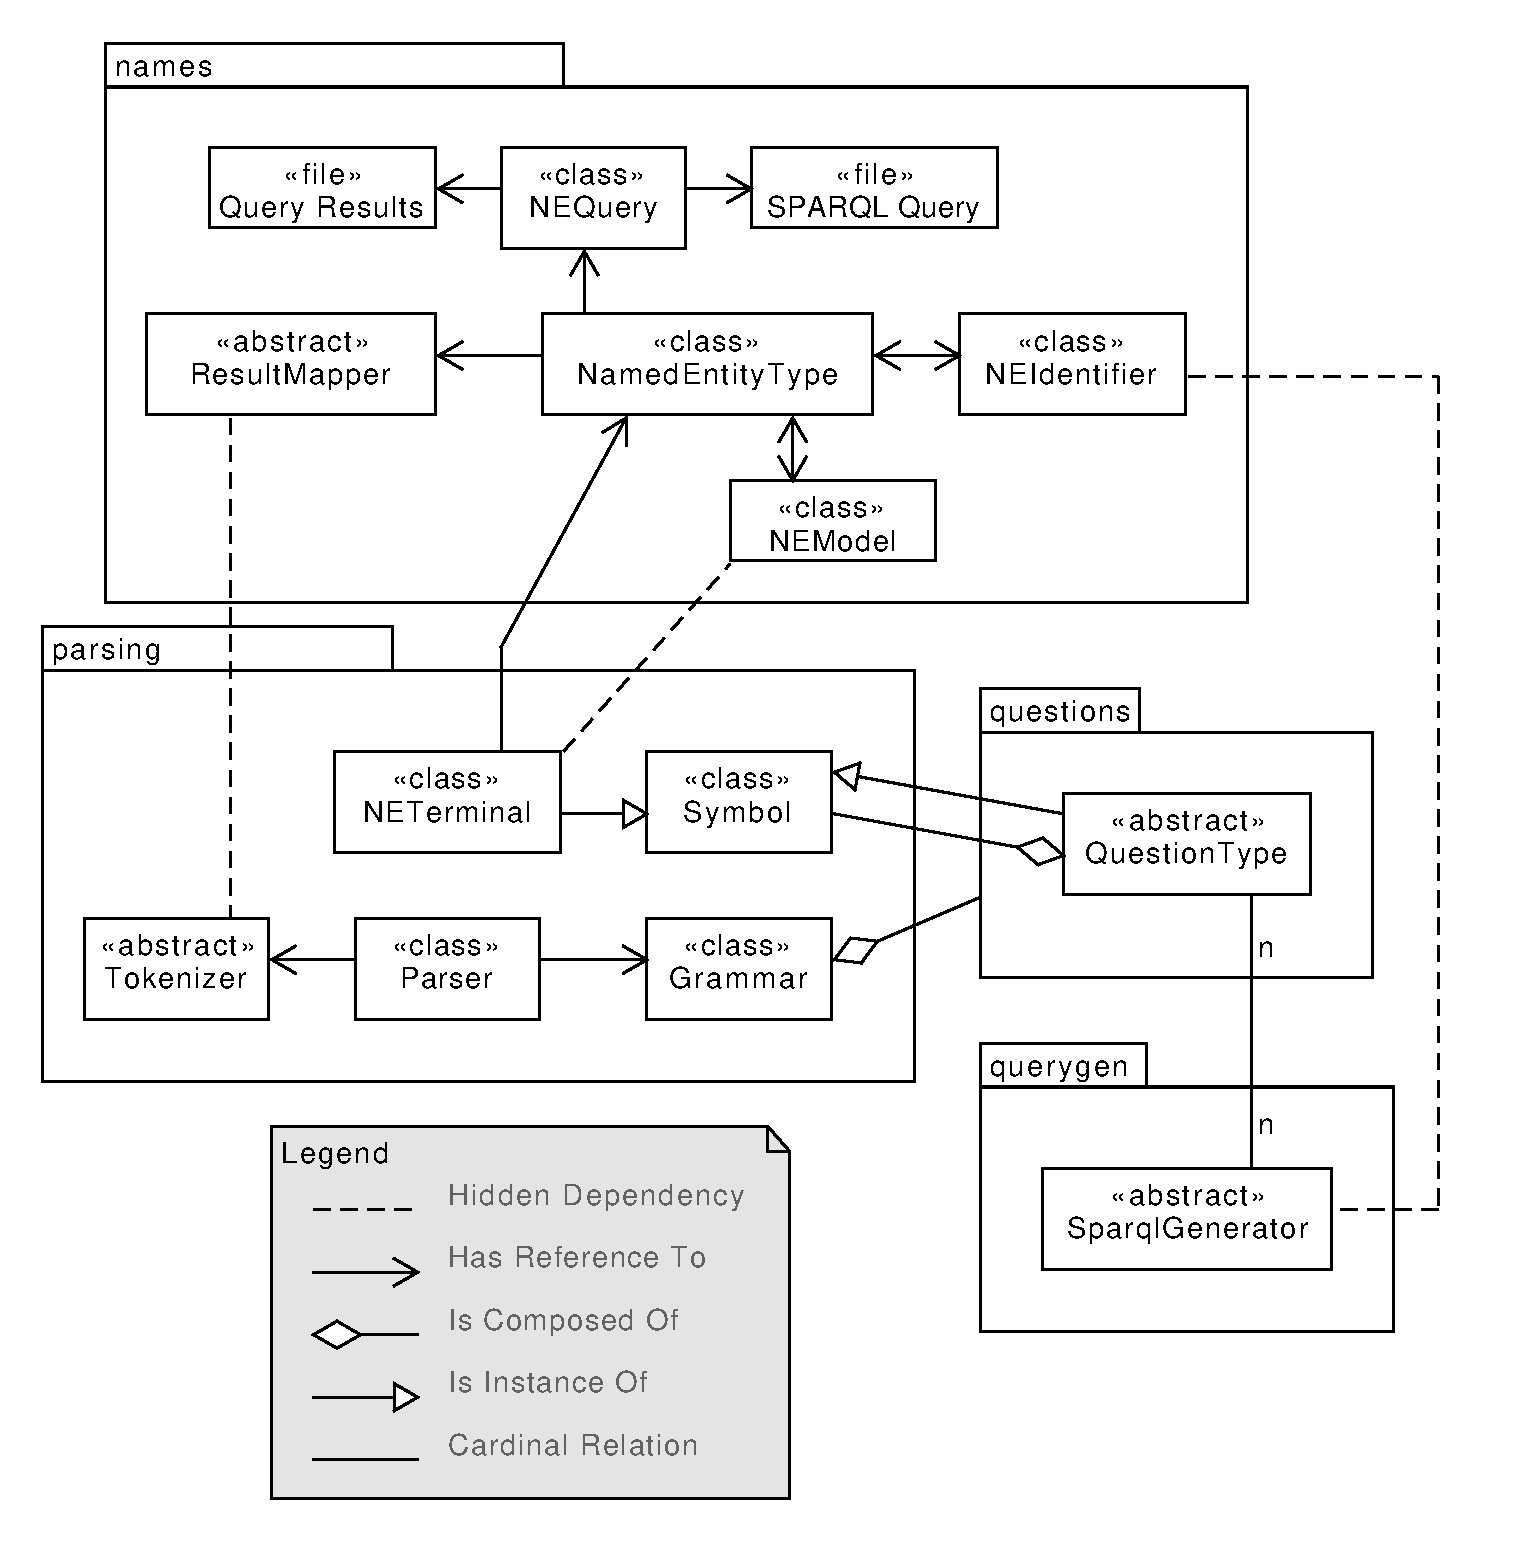
\includegraphics[width=0.9\textwidth,natwidth=1,natheight=1]{architecture.pdf}
    \caption{Architecture}
    \label{fig:arch}
\end{figure}

This architecture is aimed at handling complex questions in a narrow domain.
It does more than named entity recognition - it actually considers
the full syntax of the language. It uses
top-down parsing to generate a parse tree for the input question then
compiles SPARQL queries from that parse tree.

\begin{figure}[h!]
    \centering
    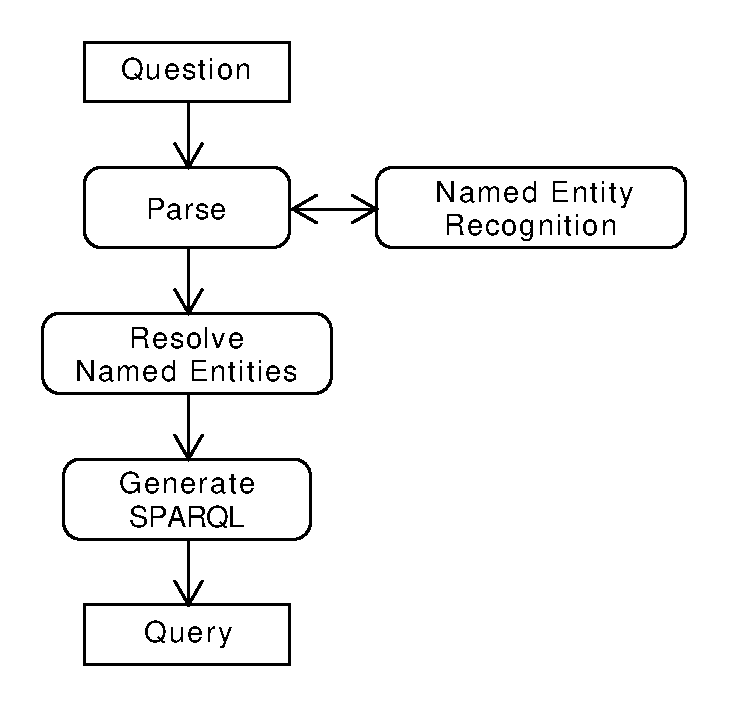
\includegraphics[width=0.9\textwidth,natwidth=1,natheight=1]{usage.pdf}
    \caption{Process}
    \label{fig:process}
\end{figure}

\section{Named Entity Recognition}
Different types of named objects are recognized as part of the parsing process.
Since the names are matched durring parsing, the NER is greatly improved by context.
Still, this matching requires a bit of preprocessing.

Statistical character models are constructed from the output of queries for all 
objects of a certain type in the target RDF database. 
These models are used to recognize arbitrary tokens (or combinations of 
tokens) within the parser's grammar. 
These particular models allow for probablistic recognition of the input strings in 
$O(1)$ time (at least, in relation to the number of objects in the RDF
database). 

%\bibliography{arch}{}
%\bibliographystyle{plain}
\end{document}
